\chapter{Python Basics}\label{app:coding}

Note to the reader: In future versions of this book we will exclusively be using Python
for the programming language of choice.  This appendix will eventually be rolled into
Chapter 1 as ``Introductory'' material that is optional for students with prior
programming experience.

In this optional Chapter we will walk through some of the basics of using Python3 - the powerful general-purpose programming language that we'll use throughout this class.  I'm assuming throughout this Chapter that you're familiar with other programming languages such as R, Java, C, or MATLAB.  Hence, I'm assuming that you know the basics about what a programming langue "is" and "does".  There are a lot of similarities between several of these languages, and in fact they borrow heavily from each other in syntax, ideas, and implementation.

We are going to be using Python in this class since

\begin{itemize}
    \item Python is free,
    \item Python is very widely used,
    \item Python is flexible,
    \item Python is relatively easy to learn,
    \item and Python is quite powerful.
\end{itemize}

It is important to keep in mind that Python is a general purpose language that we will be using for Scientific Computing.  The purpose of Scientific Computing is **not** to build apps, build software, manage databases, or develope user interfaces.  Instead, Scientific Computing is the use of a computer programming language (like Python) along with mathematics to solve scientific and mathematical problems.  For this reason it is definitely not our purpose to write an all-encompassing guide for how to use Python.  We'll only cover what is necessary for our computing needs.  You'll learn more as the course progresses so use this chapter as a reference just to get going with the language.

There is a wealth of information available about Python and the suite of tools that we will frequently use.
\begin{itemize}
    \item Python \href{https://www.python.org/}{https://www.python.org/},
    \item NumPy (numerical python) \href{https://www.numpy.org/}{https://www.numpy.org/},
    \item SciPy (scientific python) \href{https://www.scipy.org/}{https://www.scipy.org/}, and
    \item SymPy (symbolic python)
        \href{https://www.sympy.org/en/index.html}{https://www.sympy.org/en/index.html}.
\end{itemize}
These tools together provide all of the computational power that will need.  And they're free!

\section{Getting Started}
Every computer is its own unique flower with its own unique requirements.  Hence, we will
not spend time here giving you all of the ways that you can install Python and all of the
associated packages necessary for this course.  We highly recommend that you go to \\
\href{https://www.python.org/downloads/}{https://www.python.org/downloads/} and follow the
appropriate links.  The environment in which you code is largely up to personal preference
(or perhaps instructor preference).  Jupyter Notebooks seem to be a good modern choice for
coding environments.  For more information and for installation of Jupyter see
\href{https://jupyter.org/}{https://jupyter.org/}.

In the rest of this chapter we will assume that you have a working version of Python along
with (most likely) a working version of Jupyter Notebooks to work in.  Throughout this
chapter all code will be highlighted in boxes so you, the reader, can easily tell that it
is supposed to be code.  The output of the code may also be in a box.  Lastly, the code
and the output have line numbers so the reader can more easily keep track of the commands,
discuss with their peers, and discuss with their instructor.  The problems in this
appendix are
meant to get you going with the Python and you should do every one of them.  Remember that
this is not a full replacement for a ``how to program in Python'' resource.  We have only
included the essential aspects of the Python language in this chapter as they relate to
the mathematical goals of the book.  There is definitely more to say about Python and we
don't intend to cover it all here.


As is tradition for a new programming language, we should create code that prints the
words ``Hello, world!'' to the screen.  The code below does just that.  

\bcode
\begin{lstlisting}
print("Hello, world!")
\end{lstlisting}
\boutput
\begin{lstlisting}
Hello, world!
\end{lstlisting}


\begin{problem}
    Write code to print your name to the screen.
\end{problem}

Python is a general purpose programming language that can be used for all sorts of
programming tasks.  In this book we will focus on uses of Python that are more
computational and mathematical in nature.  It is expected that you already know a bit a
programming from another math class that required some coding, possibly from an
introductory computer science class, or from some other exposure to coding.  If not then
don't fret -- not all hope is lost.  A good place to start is to ask your instructor for
additional programming materials.  

\section{Python Programming Basics}
\subsection{Variables}
Variables in Python can contain letters (lower case or capital), numbers 0-9, and some
special characters such as the underscore. Variable names should start with a letter. Of
course there are a bunch of reserved words (just like in any other language). You should
look up what the reserved words are in Python so you don't accidentally use them.

You can do the typical things with variables. Assignment is with an equal sign (be careful
R users!).

{\bf Warning:} When defining numerical variables you don't always get floating point
numbers like in MATLAB. In MATLAB if you write \texttt{x=1} then automatically \texttt{x}
is saved as 1.0; a floating point decimal number, not an integer. However, in Python if
you assign \texttt{x=1} it is defined as an \underline{integer} (with no decimal digits)
but if you assign \texttt{x=1.0} it is assigned as a floating point number.

\begin{example}[Number Types in Python]

\bcode    
\begin{lstlisting}
# assign some variables
x = 7 # integer assignment of the integer 7
y = 7.0 # floating point assignment of the decimal number 7.0
print(x, type(x))
print(y, type(y))

# multiplying by a float will convert an integer to a float
print(1.0*x , type(1.0*x)) 
\end{lstlisting}
\boutput
\begin{lstlisting}
7 <class 'int'>
7.0 <class 'float'>
7.0 <class 'float'>
\end{lstlisting}
\end{example}


Note that the allowed mathematical operations are: 
\begin{itemize}
    \item Addition: \verb|+|
    \item Subtraction: \verb|-|
    \item Multiplication: \verb|*| 
    \item Division: \verb|/| 
    \item Integer Division (modular division): \verb|//| and
    \item Exponents: \verb|**|
\end{itemize}
That's right, the caret key, \verb|^|, is NOT an exponent in Python (sigh). Instead we
have to get used to \verb|**| for powers.

\begin{example}[Powers in Python]
    Keep in mind that the caret key is not an exponent in Python.  

\bcode    
\begin{lstlisting}
x = 7.0
y = x**2 # square the value in x
print(y)
\end{lstlisting}
\boutput
\begin{lstlisting}
49.0
\end{lstlisting}
\end{example}

\begin{problem}
    What happens if you type $7^2$ into Python?  What does it give you?  Can you figure
    out what it is doing?
\end{problem}

\begin{problem}
    Write code to define the variables  $a,b,$ and $c$  of your own choosing. Then
    calculate $a^2$, $b^2$, and $c^2$. When you have all three computed, check to see if
    your three values form a Pythagorean Triple so that $a^2 + b^2 = c^2$ and have Python
    simply say True or False to verify that you do, or do not, have a Pythagorean Triple
    defined.  \\
    Hint: You will need to use the == Boolean check just like in other
    programming languages.
\end{problem}



\subsection{Indexing and Lists}
Lists are a key component to storing data in Python.  Lists are exactly what the name
says: lists of things (in our case, usually the entries are floating point numbers).  

{\bf Warning to MATLAB users:} Python indexing starts at 0 whereas MATLAB indexing starts
at 1. We just have to keep this in mind.

We can extract a part of a list using the syntax [start:stop] which extracts elements
between index start and stop-1.\\
NOTE: Python stops reading at the second to last index.

Some things to keep in mind with Python lists: 
\begin{itemize}
    \item Python starts indexing at 0
    \item Python stops reading at the second to last index
    \item The following blocks of code show this feature in action for several different lists.
\end{itemize}

\begin{example}
Let's look at a few examples of indexing from lists.  In this example we will use the list
of numbers 1 through 8.
\begin{itemize}
    \item Create the list of numbers 1 through 8 and then print only the element
        with index 0.

\bcode        
\begin{lstlisting}
MyList = [1,2,3,4,5,6,7,8] 
print(MyList[0]) 
\end{lstlisting}
\boutput
\begin{lstlisting}
1
\end{lstlisting}
\item Print all elements up to, but not including, the third element.

\bcode    
\begin{lstlisting}
print(MyList[:2]) 
\end{lstlisting}
\boutput
\begin{lstlisting}
[1, 2]
\end{lstlisting}

\item Print the last element (this is a handy trick!).

\bcode
\begin{lstlisting}
print(MyList[-1]) 
\end{lstlisting}
\boutput
\begin{lstlisting}
8
\end{lstlisting}

\item Print the elements indexed 1 through 4. Beware!  This is not the first through fifth
    element.

\bcode
\begin{lstlisting}
print(MyList[1:5]) 
\end{lstlisting}
\boutput
\begin{lstlisting}
[2, 3, 4, 5]
\end{lstlisting}
\end{itemize}
\end{example}


\begin{example}
    Let's look at another example of indexing in lists.  In this one we'll use the
    \texttt{range} command to build the initial list of numbers.  Read the code carefully
    so you know what each line does.

    \bcode
\begin{lstlisting}
MySecondList = list(range(4,20)) # range is a handy command for creating a sequence of integers
print(MySecondList) # notice that it didn't create the last element!
print(MySecondList[0]) # print the first element ... the one with index 0
print(MySecondList[-5]) # print the fifth element from the end
print(MySecondList[-1:0:-1]) # print the last element to the one indexed by 1 counting backwards
print(MySecondList[::2]) # print every other element starting at the beginning
\end{lstlisting}
\boutput
\begin{lstlisting}
[4, 5, 6, 7, 8, 9, 10, 11, 12, 13, 14, 15, 16, 17, 18, 19]
4
15
[19, 18, 17, 16, 15, 14, 13, 12, 11, 10, 9, 8, 7, 6, 5]
[4, 6, 8, 10, 12, 14, 16, 18]
\end{lstlisting}
\end{example}

In Python, elements in a list do not need to be the same type. You can mix integers,
floats, strings, lists, etc.
\begin{example}[Lists with elements of mixed type]
    In this example we see a list of several items that have different data types: float,
    integer, string, and complex.  Note that the imaginary number $i$ is represented by
    $j$ in Python.  This is common in many scientific disciplines and is just another
    thing that we'll need to get used to in Python.

    \bcode
\begin{lstlisting}
MixedList = [1.0, 7, 'Bob', 1-1j]
print(MixedList)
print(type(MixedList[0]))
print(type(MixedList[1]))
print(type(MixedList[2]))
print(type(MixedList[3])) # Notice that we use 1j for the imaginary number "i".
\end{lstlisting}
\boutput
\begin{lstlisting}
[1.0, 7, 'Bob', (1-1j)]
<class 'float'>
<class 'int'>
<class 'str'>
<class 'complex'>
\end{lstlisting}
\end{example}

\begin{problem}
    \begin{enumerate}
        \item[(a)] Create the list of the first several Fibonacci numbers:\\
            $1, 1, 2, 3, 5, 8, 13, 21, 34, 55, 89$.
        \item[(b)] Print the first four elements of the list.
        \item[(c)] Print every third element of the list.
        \item[(d)] Print the last element of the list.
    \end{enumerate}
\end{problem}

\subsection{List Operations}
Python is awesome about allowing you to do things like appending items to lists, removing
items from lists, and inserting items into lists.  Note in all of the examples below that
we are using the code \\\texttt{variable.command}\\ where you put the variable name, a dot,
and the thing that you would like to do to that variable.  For example,
\texttt{MyList.append(7)} will append the number 7 to the list \texttt{MyList}.  This is a
common programming feature in Python and we'll use it often.

\begin{example}[Appending To Lists]
    The \texttt{.append} command can be used to append an element to the end of a list.

    \bcode
\begin{lstlisting}
MyList = [0,1,2,3]
print(MyList)
MyList.append('a') # append the string 'a' to the end of the list
print(MyList)
MyList.append('a') # do it again ... just for kicks
print(MyList)
MyList.append(15) # append the number 15 to the end of the list
print(MyList)
\end{lstlisting}
\boutput
\begin{lstlisting}
[0, 1, 2, 3]
[0, 1, 2, 3, 'a']
[0, 1, 2, 3, 'a', 'a']
[0, 1, 2, 3, 'a', 'a', 15]
\end{lstlisting}
\end{example}

\begin{example}[Removing From Lists]
    The \texttt{.remove} command can be used to remove an element from a list.

    \bcode
\begin{lstlisting}
MyList.remove('a') # remove the first instance of the string `a` from the list
print(MyList)
MyList.remove(3) # now let's remove the 3
print(MyList)
\end{lstlisting}
\boutput
\begin{lstlisting}
[0, 1, 2, 3, 'a', 15]
[0, 1, 2, 'a', 15]
\end{lstlisting}
\end{example}

\begin{example}[Inserting Into Lists]
    The \texttt{.insert} command can be used to insert an element at a location in a list.

    \bcode
\begin{lstlisting}
MyList.insert(0,'A') # insert the letter `A` at the 0-indexed spot
MyList.insert(3,'B') # insert the letter `B` at the spot with index 3 
# remember that index 3 means the fourth spot in the list
print(MyList)
\end{lstlisting}
\boutput
\begin{lstlisting}
['A', 0, 1, 'B', 2, 'a', 15]
\end{lstlisting}
\end{example}

\begin{problem}
    \begin{enumerate}
        \item[(a)] Create the list of the first several Lucas Numbers: \\
            $1,3,4,7,11,18,29,47.$
        \item[(b)] Add the next three Lucas Numbers to the end of the list.
        \item[(c)] Remove the number 3 from the list.
        \item[(d)] Insert the 3 back into the list in the correct spot.
        \item[(e)] Print the list in reverse order (how do you suppose you should do this?)
        \item[(f)] Do a few other list operations to this list and report your findings.
    \end{enumerate}
\end{problem}

\subsection{Tuples}
In Python, a "tuple" is like an ordered pair (or order triple, or order quadruple, ...) in
mathematics.  We will occasionally see tuples in our work in numerical analysis so for now
let's just give a couple of code snippets showing how to store and read them.

\begin{example}[Defining Tuples]
    We can define the tuple of numbers $(10,20)$ in Python as follows.

    \bcode
\begin{lstlisting}
point = 10, 20 # notice that I don't need the parenthesis
print(point, type(point))
\end{lstlisting}
\boutput
\begin{lstlisting}
(10, 20) <class 'tuple'>
\end{lstlisting}

We can also define the type with parenthesis if we like.  Python doesn't care.

\bcode
\begin{lstlisting}
point = (10, 20) # now we define the tuple with parenthesis
print(point, type(point))
\end{lstlisting}
\boutput
\begin{lstlisting}
(10, 20) <class 'tuple'>
\end{lstlisting}
\end{example}



\begin{example}[Unpacking Tuples]
 The cool thing is that we can then unpack the tuple into components if we wish.   
 \bcode
\begin{lstlisting}
x, y = point
print("x = ", x)
print("y = ", y)
\end{lstlisting}
\boutput
\begin{lstlisting}
x =  10
y =  20
\end{lstlisting}
\end{example}



\subsection{Control Flow: Loops and If Statements}
Just like in other programming languages we can do loops and conditional statements in
very easy ways. The thing to keep in mind is that Python is very white-space-dependent.
This means that your indentations need to be correct in order for a loop to work. You
could get away with sloppy indention in other languages (like MATLAB) but not so in
Python. Also, in some languages (like R and Java) you need to wrap your loops in curly
braces. Again, not so in Python.

{\bf Caution:} Be really careful of the white space in your code when you write loops.

\subsubsection{For Loops}
A for loop is designed to do a task a certain number of times and then stop. This is a
great tool for automating repetitive tasks, but it also nice numerically for building
sequences, summing series, or just checking lots of examples. The following are several
examples of Python for loops. Take careful note of the syntax for a for loop as it is the
same as for other loops and conditional statements:

\begin{itemize}
    \item a control statement,
    \item a colon, a new line,
    \item indent four spaces,
    \item some programming statements
\end{itemize}
When you are done with the loop just back out of the indention. There is no need for an
``end'' command or a curly brace. All of the control statements in Python are
white-space-dependent.

\begin{example}
    Print the first 6 perfect square.

    \bcode
\begin{lstlisting}
for x in [1,2,3,4,5,6]:
    print(x**2)
\end{lstlisting}
\boutput
\begin{lstlisting}
1.0
4.0
9.0
16.0
25.0
36.0
\end{lstlisting}
\end{example}

\begin{example}
Print the names in a list.

\bcode
\begin{lstlisting}
NamesList = ['Alice','Billy','Charlie','Dom','Enrique','Francisco']
for name in NamesList:
    print(name)
\end{lstlisting}
\boutput
\begin{lstlisting}
Alice
Billy
Charlie
Dom
Enrique
Francisco
\end{lstlisting}
\end{example}

You can use a more compact notation sometimes. This takes a bit of getting used to, but is
super slick!

\begin{example}
Create a list of the perfect squares from 1 to 9.

\bcode
\begin{lstlisting}
# create a list of the perfect squares from 1 to 9
CoolList = [x**2 for x in range(1,10)]
print(CoolList)
# Then print the sum of this list
print("The sum of the first 9 perfect squares is",sum(CoolList))
\end{lstlisting}
\boutput
\begin{lstlisting}
[1, 4, 9, 16, 25, 36, 49, 64, 81]
The sum of the first 9 perfect squares is 285
\end{lstlisting}
\end{example}

For loops can also be used to build recursive sequences as can be seen in the next couple
of examples.

\begin{example}
    In the following code we write a for loop that outputs a list of the first 10
    iterations of the sequence  $x_{n+1}=−0.5x_n+1$ starting with  $x_0=3$. Notice that
    we're using \texttt{x.append} instead of $x[n+1]$ to append the new term to the list.
    This allows us to grow the length of the list dynamically as the loop progresses.

    \bcode
\begin{lstlisting}
x=[3.0]
for n in range(0,9):
    x.append(-0.5*x[n] + 1)
print(x)
\end{lstlisting}
\boutput
\begin{lstlisting}
[3.0, -0.5, 1.25, 0.375, 0.8125, 0.59375, 0.703125, 0.6484375, 
    0.67578125, 0.662109375]
\end{lstlisting}
\end{example}
As an alternative to the code immediately above we can pre-allocate the memory in an array
of zeros. This is done with the clever code \texttt{x = [0] * 10}. Literally multiplying a
list by some number, like 10, says to repeat that list 10 times.

\begin{example}
    Now we'll build the sequence with pre-allocated memory.

    \bcode
\begin{lstlisting}
x = [0] * 10
x[0] = 3.0
for n in range(0,9):
    x[n+1] = -0.5*x[n]+1
    print(x) # This print statement shows x at each iteration
\end{lstlisting}
\boutput
\begin{lstlisting}
[3.0, -0.5, 0, 0, 0, 0, 0, 0, 0, 0]
[3.0, -0.5, 1.25, 0, 0, 0, 0, 0, 0, 0]
[3.0, -0.5, 1.25, 0.375, 0, 0, 0, 0, 0, 0]
[3.0, -0.5, 1.25, 0.375, 0.8125, 0, 0, 0, 0, 0]
[3.0, -0.5, 1.25, 0.375, 0.8125, 0.59375, 0, 0, 0, 0]
[3.0, -0.5, 1.25, 0.375, 0.8125, 0.59375, 0.703125, 0, 0, 0]
[3.0, -0.5, 1.25, 0.375, 0.8125, 0.59375, 0.703125, 0.6484375, 0, 0]
[3.0, -0.5, 1.25, 0.375, 0.8125, 0.59375, 0.703125, 0.6484375, 0.67578125, 0]
[3.0, -0.5, 1.25, 0.375, 0.8125, 0.59375, 0.703125, 0.6484375, 0.67578125, 0.662109375]
\end{lstlisting}
\end{example}

\begin{problem}
    We want to sum the first 100 perfect cubes. Let's do this in two ways.

    \begin{enumerate}
        \item Start off a variable called Total at 0 and write a for loop that adds the
            next perfect cube to the running total.
        \item  Write a for loop that builds the sequence of the first 100 perfect cubes.
            After the list has been built find the sum with the sum command.
    \end{enumerate}
    The answer is: 25,502,500 so check your work.
\end{problem}

\begin{problem}
    Write a for loop that builds the first 20 terms of the sequence  $x_{n+1}=1−x^2$ with
    $x_0=0.1$ Pre-allocate enough memory in your list and then fill it with the terms of
    the sequence. Only print the list after all of the computations have been completed.
\end{problem}

\subsubsection{While Loops}
A while loop repeats some task (or sequence of tasks) until a logical condition is met.
The structure in Python is the same as with for loops.

\begin{example}
    Print the numbers 0 through 4 and then the word ``done''. We'll do this by starting a
    counter variable, \texttt{i}, at 0 and incrementing it every time we pass through the
    loop.

    \bcode
\begin{lstlisting}
i = 0
while i < 5:
    print(i)
    i += 1 # increment the counter
print("done")
\end{lstlisting}
\boutput
\begin{lstlisting}
0
1
2
3
4
done
\end{lstlisting}
\end{example}

\begin{example}
    Now let's use a while loop to build the sequence of Fibonacci numbers and stop when
    the newest number in the sequence is greater than 1000. Notice that we want to keep
    looping until the condition that the last term is greater than 1000 -- this is the
    perfect task for a while loop, instead of a for loop, since we don't know how many steps
    it will take before we start the task

    \bcode
\begin{lstlisting}
Fib = [1,1]
while Fib[-1] <= 1000:
    Fib.append(Fib[-1] + Fib[-2])
Fib
\end{lstlisting}
\boutput
\begin{lstlisting}
[1, 1, 2, 3, 5, 8, 13, 21, 34, 55, 89, 144, 233, 377, 610, 987, 1597]
\end{lstlisting}

\end{example}

\begin{problem}
    Write a while loop that sums the terms in the Fibonacci sequence until the sum is
    larger than 1000
\end{problem}


\subsubsection{If Statements}
Conditional (if) statements allow you to run a piece of code only under certain
conditions.  This is handy when you have different tasks to perform under different
conditions.  

\begin{example}
    
    \bcode
\begin{lstlisting}
Name = "Alice"
if Name == "Alice":
    print("Hello, Alice.  Isn't it a lovely day to learn Python?")
else:
    print("You're not Alice.  Where is Alice?")
\end{lstlisting}
\boutput
\begin{lstlisting}
Hello, Alice.  Isn't it a lovely day to learn Python?
\end{lstlisting}
\bcode
\begin{lstlisting}
Name = "Billy"
if Name == "Alice":
    print("Hello, Alice.  Isn't it a lovely day to learn Python?")
else:
    print("You're not Alice.  Where is Alice?")
\end{lstlisting}
\boutput
\begin{lstlisting}
You're not Alice.  Where is Alice?
\end{lstlisting}
\end{example}

\begin{example}
    For another example, if we get a random number between 0 and 1 we could have Python
    print a different message depending on whether it was above or below 0.5. Run the code
    below several times and you'll see different results each time.

    Note: We had to import the \texttt{numpy} package to get the random number generator
    in Python.  Don't worry about that for now.  We'll talk about packages in a moment.

    
    \bcode
\begin{lstlisting}
import numpy as np
x = np.random.rand(1,1) # get a random 1x1 matrix using numpy
x = x[0,0] # pull the entry from the first row, first column of the random matrix
if x < 0.5:
    print(x," is less than a half")
else:
    print(x, "is NOT less than a half")
\end{lstlisting}
\boutput
\begin{lstlisting}
0.654697487883 is NOT less than a half
\end{lstlisting}
(Take note that the output will change every time you run it)
\end{example}

In many programming tasks it is handy to have several different choices between tasks
instead of just two choices as in the previous examples.  This is a job for the
\texttt{elif} command.

\begin{example}
This is the same code as last time except we will make the decision at 0.33 and 0.67    
\bcode
\begin{lstlisting}
import numpy as np
x = np.random.rand(1,1) # get a random 1x1 matrix using numpy
x = x[0,0] # pull the entry from the first row, first column of the random matrix
if x < 0.33:
    print(x," is less than one third")
elif x < 0.67:
    print(x, "is less than two thirds but greater than or equal to one third")
else:
    print(x, "is greater than or equal to two thirds")
\end{lstlisting}
\boutput
\begin{lstlisting}
0.654697487883 is less than two thirds but greater than or equal to one third
\end{lstlisting}
(Take note that the output will change every time you run it)
\end{example}

\begin{problem}
    Write code to give the Collatz Sequence
$$x_{n+1} = \left\{ \begin{array}{ll} x_n / 2, & \text{$x_n$ is even} \\ 3 x_n + 1, & \text{otherwise} \end{array} \right.$$
starting with a positive integer of your choosing.  The sequence will converge to 1 so your code should stop when the sequence reaches 1.

\end{problem}





\subsection{Functions}
Mathematicians and programmers talk about functions in very similar ways, but they aren't
exactly the same.  When we say ``function'' in a programming sense we are talking about a
chunk of code that you can pass parameters and expect an output of some sort.  This is not
unlike the mathematician's version, but unlike a mathematical function we can have
multiple outputs for a programmatic function.  We are not going to be talking about
symbolic computation on functions in this section.  Symbolic computations will have to
wait for the `sympy` tutorial.



In Python, to define a function we start with \texttt{def}, followed by the function's
name, any input variables in parenthesis, and a colon.  The indented code after the colon
is what defines the actions of the function.

\begin{example}
The following code defines the polynomial $f(x) = x^3 + 3x^2 + 3x + 1$ and then evaluates
the function at a point $x=2.3$.

\bcode
\begin{lstlisting}
def f(x):
    return(x**3 + 3*x**2 + 3*x + 1)
f(2.3)
\end{lstlisting}
\boutput
\begin{lstlisting}
35.937
\end{lstlisting}
\end{example}
Take careful note of several things in the previous example:
\begin{itemize}
    \item To define the function we can not just type it like we would see it one paper.
        This is not how Python recognizes functions.  We just have to get used to it.
        Other scientific programming languages will allow you to define mathematical
        functions in this way, but Python will not.
    \item Once we have the function defined we can call upon it just like we would on
        paper.
    \item We cannot pass symbols into this type of function.  See the section on
        \texttt{sympy} in this chapter if you want to do symbolic computation.
\end{itemize}


\begin{problem}
    Define the function $g(n) = n^2 + n + 41$ as a Python function.  Write a loop that
    gives the output for this function for integers from $n=0$ to $n=39$.  It is curious
    to note that each of these outputs is a prime number (check this on your own).  Will
    the function produce a prime for $n=40$? For $n=41$?  
\end{problem}

One cool thing that you can do with Python functions is call them recursively.  That is,
you can call the same function from within the function itself.  This turns out to be
really handy in several mathematical situations.

\begin{example}
    Now let's define a function for the factorial. This function is naturally going to be
    recursive in the sense that it calls on itself!

    \bcode
\begin{lstlisting}
def Fact(n):
    if n==0:
        return(1)
    else:
        return( n*Fact(n-1) ) # we are calling the same function recursively.
\end{lstlisting}
When you run this code there will be no output.  You have just defined the function so you
can use it later.  So let's use it to make a list of the first several factorials.  Note
the use of a for loop in the following code.

\bcode
\begin{lstlisting}
FactList = [Fact(n) for n in range(0,10)]
FactList
\end{lstlisting}
\boutput
\begin{lstlisting}
[1, 1, 2, 6, 24, 120, 720, 5040, 40320, 362880]
\end{lstlisting}
\end{example}


\begin{example}
    For this next example let's define the sequence 
$$x_{n+1} = \left\{ \begin{array}{ll} 2x_n, & x_n \in [0,0.5] \\ 2x_n - 1, & x_n \in (0.5,1] \end{array} \right.$$ 
as a function and then build a loop to find the first several iterates of the sequence starting at any real number between 0 and 1.

\bcode
\begin{lstlisting}
# Define the function
def MySeq(xn):
    if xn <= 0.5:
        return(2*xn)
    else:
        return(2*xn-1)

# Now build a sequence with this function
x = [0.125] # arbitrary starting point
for n in range(0,5): # Let's only build the first 5 terms
    x.append(MySeq(x[-1]))
print(x)
\end{lstlisting}
\boutput
\begin{lstlisting}
[0.125, 0.25, 0.5, 1.0, 1.0, 1.0]
\end{lstlisting}
\end{example}


\begin{example}
    Here is another cool example.

A fun way to approximate the square root of two is to start with any positive real number
and iterate over the sequence 
$$x_{n+1} = \frac{1}{2} x_n + \frac{1}{x_n}$$ 
until we are
within any tolerance we like of the square root of two.  Write code that defines the
sequence as a function and then iterates in a while loop until we are within $10^{-8}$ of
the square root of 2.  

Hint: Import the \texttt{math} package so that you get the square root.  More about
packages in the next section.

\bcode
\begin{lstlisting}
from math import sqrt
def f(x):
    return(0.5*x + 1/x)
x = 1.1 # arbitrary starting point
print("approximation \t\t exact \t\t abs error")
while abs(x-sqrt(2)) > 10**(-8):
    x = f(x)
    print(x, sqrt(2), abs(x - sqrt(2)))
\end{lstlisting}
\boutput
\begin{lstlisting}
approximation 		 exact 		 abs error
1.459090909090909 1.4142135623730951 0.04487734671781385
1.414903709997168 1.4142135623730951 0.0006901476240728233
1.4142137306897584 1.4142135623730951 1.6831666327377093e-07
1.4142135623731051 1.4142135623730951 9.992007221626409e-15
\end{lstlisting}
\end{example}

\begin{problem}
    The previous example is a special case of the Babylonian Algorithm for calculating square roots.  If you want the square root of $S$ then iterate the sequence
$$x_{n+1} = \frac{1}{2} \left( x_n + \frac{S}{x_n} \right)$$
until you are within an appropriate tolerance.

Modify the code given in the previous example to give a list of approximations of the square roots of the natural numbers 2 through 20, each to within $10^{-8}$.  This problem will require that you build a function, write a `for` loop (for the integers 2-20), and write a `while` loop inside your `for` loop to do the iterations.
\end{problem}



\subsection{Packages}
Unlike mathematical programming languages like MATLAB, Maple, or Mathematica, where every
package is already installed and ready to use, Python allows you to only load the packages
that you might need for a given task.\footnote{If you are familiar with the statistical
    programming language, R, then you might be used to the idea of importing packages or
libraries for certain tasks.}  There are several advantages to this along with a
few disadvantages.

{\bf Advantages:}
\begin{enumerate}
    \item You can have the same function doing different things in different scenarios.
        For example, there could be a symbolic differentiation command and a numerical
        differentiation command comming from different packages that are used in different
        ways.
    \item Housekeeping.  It is highly advantageous to have a good understanding of where
        your functions come from.  MATLAB uses the same name for multiple purposes with no
        indication of how it might behave depending on the inputs.  With Python you can
        avoid that by only importing the appropriate packages for your current use.
    \item Your code will be ultimately more readable (more on this later).
\end{enumerate}

{\bf Disadvantages:}
\begin{enumerate}
    \item It is often challenging to keep track of which function does which task when
        they have exactly the same name.  For example, you could be working with the
        \texttt{sin()} function numerically from the \texttt{numpy} package or
        symbolically from the \texttt{sympy} package, and these functions will behave differently in Python - even though they are exactly the same mathematically.
    \item You need to remember which functions live in which packages so that you can load the right ones.  It is helpful to keep a list of commonly used packages and functions at least while you're getting started.
\end{enumerate}

Let's start with the \texttt{math} package.    

\begin{example}[Importing the \texttt{math} Package]
The code below imports the \texttt{math}
package into your instance of Python and calculates the cosine of $\pi/4$.

\bcode
\begin{lstlisting}
import math
x = math.cos(math.pi / 4)
print(x)
\end{lstlisting}
\boutput
\begin{lstlisting}
0.7071067811865476
\end{lstlisting}
The answer, unsurprisingly, is the decimal form of $\sqrt{2}/2$.
\end{example}

You might already see a potential disadvantage: there is now more typing involved! Let's
fix this.  When you import a package you could just import all of the functions so they
can be used by their proper names.

\begin{example}
    Here we import the entire math package so we can use every one of the functions
    therein without having to use the \texttt{math} prefix.

    \bcode
\begin{lstlisting}
from math import * # read this as: from math import everything
x = cos(pi / 4)
print(x)
\end{lstlisting}
\boutput
\begin{lstlisting}
0.7071067811865476
\end{lstlisting}
The end result is exactly the same: the decimal form of $\sqrt{2}/2$, but now we had less
typing to do.
\end{example}

Now you can freely use the functions that were imported from the math package. There is a
disadvantage to this, however. What if we have two packages that import functions with the
same name. For example, in the \texttt{math} package and in the \texttt{numpy} package
there is a \texttt{cos()} function. In the next block of code we'll import both
\texttt{math} and \texttt{numpy}, but instead we will import them with shortened names so
we can type things a bit faster.

\begin{example}[Importing Multiple Packages]
    Here we import \texttt{math} and \texttt{numpy} under aliases so we can use the
    shortened aliases and not mix up which functions belong to which packages.

    \bcode
\begin{lstlisting}
import math as ma
import numpy as np
x = ma.cos( ma.pi / 4) # use the math version of the cosine function
y = np.cos( np.pi / 4) # use the numpy version of the cosine function
print(x, y)
\end{lstlisting}
\boutput
\begin{lstlisting}
0.7071067811865476 0.707106781187
\end{lstlisting}
Both ``x'' and ``y'' in the code give the decimal approximation of $\sqrt{2}/2$.  This is
clearly pretty redundant in this really simple case, but you should be able to see where
you might want to use this and where you might run into troubles.
\end{example}


Once you have a package imported you can see what is inside of it using the \texttt{dir}
command.  

\begin{example}[Looking Inside a Package]
    The following block of code prints a list of all of the functions inside the
\texttt{math} package.

\bcode
\begin{lstlisting}
import math
print(dir(math))
\end{lstlisting}
\boutput
\begin{lstlisting}
['__doc__', '__file__', '__loader__', '__name__', '__package__',
'__spec__', 'acos', 'acosh', 'asin', 'asinh', 'atan', 'atan2', 
'atanh', 'ceil', 'copysign', 'cos', 'cosh', 'degrees', 'e', 'erf', 
'erfc', 'exp', 'expm1', 'fabs', 'factorial', 'floor', 'fmod', 
'frexp', 'fsum', 'gamma', 'gcd', 'hypot', 'inf', 'isclose', 
'isfinite', 'isinf', 'isnan', 'ldexp', 'lgamma', 'log', 'log10', 
'log1p', 'log2', 'modf', 'nan', 'pi', 'pow', 'radians', 'sin', 
'sinh', 'sqrt', 'tan', 'tanh', 'tau', 'trunc']
\end{lstlisting}
\end{example}

Of course, there will be times when you need help with a function.  You can use the
\texttt{help} command to view the help documentation for any function.  

\begin{example}[Help]
    Here we get help on the arc cosine function in the \texttt{math} package.

    \bcode
\begin{lstlisting}
help(math.acos)
\end{lstlisting}
\boutput
\begin{lstlisting}
Help on built-in function acos in module math:
acos(...)
    acos(x)
    Return the arc cosine (measured in radians) of x.
\end{lstlisting}
\end{example}

\begin{problem}
    Import the math package, figure out how the \texttt{log} function works, and write
    code to calculate the logarithm of the number 8.3 in base 10, base 2, base 16, and
    base $e$  (the natural logarithm).
\end{problem}





\section{Numerical Python with \texttt{numpy}}
The base implementation of Python includes the basic programming language, the tools to
write loops, check conditions, build and manipulate lists, and all of the other things
that we saw in the previous section.  In this section we will explore the package
\texttt{numpy} that contains optimized numerical routines for doing numerical computations
in scientific computing.

\begin{example}[Horrible Numerical Operations]

To start with let's look at a really simple example.  Say you have a list of real numbers
and you want to take the sine every element in the list.  If you just try to take the sine
of the list you will get an error as you can see below.

\bcode
\begin{lstlisting}
from math import pi, sin
MyList = [0,pi/6, pi/4, pi/3, pi/2, 2*pi/3, 3*pi/4, 5*pi/6, pi]
sin(MyList)
\end{lstlisting}
\boutput
\begin{lstlisting}
TypeError: must be real number, not list
\end{lstlisting}
You could get around this error using some of the tools from base Python, but none of them
are very elegant from a programming perspective.  

\bcode
\begin{lstlisting}
SineList = [sin(n) for n in MyList]
print(SineList)
\end{lstlisting}
\boutput
\begin{lstlisting}
[0.0, 0.49999999999999994, 0.7071067811865475, 0.8660254037844386, 
1.0, 0.8660254037844388, 0.7071067811865476, 0.49999999999999994, 
1.2246467991473532e-16]
\end{lstlisting}

\bcode
\begin{lstlisting}
SineList = [ ]
for n in range(0,len(MyList)):
    SineList.append( sin(MyList[n]) )
SineList
\end{lstlisting}
\boutput
\begin{lstlisting}
[0.0,
 0.49999999999999994,
 0.7071067811865475,
 0.8660254037844386,
 1.0,
 0.8660254037844388,
 0.7071067811865476,
 0.49999999999999994,
 1.2246467991473532e-16]
\end{lstlisting}

\end{example}

The package \texttt{numpy} is used in almost all numerical computations using Python.  It
provides algorithms for matrix and vector arithmetic.  Furthermore, it is optimized to be
able to do these computations in the most efficient possible way (both in terms of memory
and in terms of speed).

Typically when we import \texttt{numpy} we use \texttt{import numpy as np}.  This is the
standard way to name the \texttt{numpy} package.  This means that we will have lots of
function with the prefix ``np'' in order to call on the \texttt{numpy} commands.  Let's
first see what is inside the package.  A brief glimpse through the following list reveals
a huge wealth of mathematical functions that are optimized to work in the best possible
way with the Python language. (we are intentionally not showing the output here since it
is quite extensive)

\bcode
\begin{lstlisting}
import numpy as np
# Uncomment the next line of code and run it.  
# print(dir(np)) 
\end{lstlisting}




\subsection{Numpy Arrays, Array Operations, and Matrix Operations}
In the previous section you worked with Python lists.  As we pointed out, the shortcoming
of Python lists is that they don't behave well when we want to apply mathematical
functions to the vector as a
whole.  The "numpy array", \texttt{np.array}, is essentially the same as a Python list with the
notable exception that

\begin{itemize}
    \item In a \texttt{numpy} array every entry is a floating point number
    \item In a \texttt{numpy} array the memory usage is more efficient (mostly since
        Python is expecting data of all the same type)
    \item With a \texttt{numpy} array there are ready-made functions that can act directly
        on the array as a matrix or a vector
\end{itemize}

Let's just look at a few example.  What we're going to do is to define a matrix $A$ and vectors $v$ and $w$ as
$$A = \begin{pmatrix} 1 & 2 \\ 3 & 4 \end{pmatrix}, \quad v = \begin{pmatrix} 5\\6 \end{pmatrix}
\quad \text{and} \quad w = v^T = \begin{pmatrix} 5 & 6 \end{pmatrix}.$$
Then we'll do the following

\begin{itemize}
    \item Get the size and shape of these arrays
    \item Get individual elements, rows, and columns from these arrays
    \item Treat these arrays as with linear algebra to
        \begin{itemize}
            \item do element-wise multiplication
            \item do matrix a vector products
            \item do scalar multiplication
            \item take the transpose of matrices
            \item take the inverse of matrices
        \end{itemize}
\end{itemize}


\begin{example}[Defining Matrices and Vectors]
    The first thing to note is that a matrix is a list of lists (each row is a list).

\bcode
\begin{lstlisting}
A = np.array([[1,2],[3,4]])
print(A)
v = np.array([[5],[6]]) # this creates a column vector
print(v)
w = np.array([5,6]) # this creates a row vector
print(w)
\end{lstlisting}
\boutput
\begin{lstlisting}
[[1 2]
 [3 4]]
[[5]
 [6]]
[5 6]
\end{lstlisting}
\end{example}

\begin{example}[Shape Matrices and Vectors]
    The \texttt{variable.shape} command can be used to give the shape of a numpy array.
    Notice that the output is a tuple showing the size (rows, columns).  Also notice that
    the row vector doesn't give (1,2) as expected.  Instead it just gives (2,).  

\bcode
\begin{lstlisting}
print(A.shape) # Shape of the matrix A
print(v.shape) # Shape of the column vector v
print(w.shape) # Shape of the row vector w
\end{lstlisting}
\boutput
\begin{lstlisting}
(2, 2)
(2, 1)
(2,)
\end{lstlisting}
\end{example}

\begin{example}[Size of Matrices and Vectors]
    The \texttt{variable.size} command can be used to give the size of a numpy array.
    The size of a matrix or vector will be the total number of elements in the array.  You
    can think of this as the product of the values in the tuple coming from the shape
    command.

\bcode
\begin{lstlisting}
print(A.size) # Size (number of elements) of A
print(v.size) # Size (number of elements) of v
print(w.size) # Size (number of elements) of w
\end{lstlisting}
\boutput
\begin{lstlisting}
4
2
2
\end{lstlisting}
    
\end{example}

Reading individual elements from a \texttt{numpy} array is the same, essentially, as
reading elements from a Python list.  We will use square brackets to get the row and
column.  Remember that the indexing all starts from 0, not 1!

\begin{example}[Reading Entries from a Matrix]
    Let's read the top left and bottom right entries of the matrix $A$.

\bcode
\begin{lstlisting}
print(A)
print(A[0,0]) # top left
print(A[1,1]) # bottom right
\end{lstlisting}
\boutput
\begin{lstlisting}
[[1 2]
 [3 4]]
1
4
\end{lstlisting}
    
\end{example}

\begin{example}[Reading a Row from a Matrix]
    Let's read the first row from that matrix $A$.

\bcode
\begin{lstlisting}
print(A)
print(A[0,:])
\end{lstlisting}
\boutput
\begin{lstlisting}
[[1 2]
 [3 4]]
[1 2]
\end{lstlisting}
\end{example}


\begin{example}[Reading a Column from a Matrix]
    Let's read the second column from the matrix $A$.

\bcode
\begin{lstlisting}
print(A)
print(A[:,1])
\end{lstlisting}
\boutput
\begin{lstlisting}
[[1 2]
 [3 4]]
[2 4]
\end{lstlisting}
Notice when we read the column it was displayed as a column.  Be careful.

\end{example}

If we try to multiply either $A$ and $v$ or $A$ and $A$ we will get some funky results.
Unlike programming languages like MATLAB, the default notion of multiplication is NOT
matrix multiplication.  Instead, the default is element-wise multiplication.

\begin{example}[Element-wise Matrix Multiplication]
    If we write the code \texttt{A*A} we do NOT do matrix multiplication.  Instead we do
    element-by-element multiplication.  This is a common source of issues when dealing
    with matrices and linear algebra in Python.

\bcode
\begin{lstlisting}
print(A)
A * A # Notice that this is NOT the same as A*A with matrix multiplication
\end{lstlisting}
\boutput
\begin{lstlisting}
[[1 2]
[3 4]]
array([[ 1,  4],
       [ 9, 16]])
\end{lstlisting}
\end{example}

\begin{example}[Element-wise Matrix-Vector Multiplication]
    If we write \texttt{A * v} Python will do element-wise multiplication across each
    column since $v$ is a column vector.

\bcode
\begin{lstlisting}
print(A)
print(v)
A * v # This will actually do element wise multiplication on each column
\end{lstlisting}
\boutput
\begin{lstlisting}
[[1 2]
 [3 4]]
[[5]
 [6]]
array([[ 5, 10],
       [18, 24]])
\end{lstlisting}

\end{example}

If, however, we recast these arrays as matrices we can get them to behave as we would
expect from Linear Algebra. It is up to you to check that these products are indeed
correct from the definitions of matrix multiplication from Linear Algebra.

\begin{example}[Matrix-Matrix and Matrix-Vector Multiplication]
    Recasting the numpy arrays as matrices allows you to use multiplication as we would
    expect from linear algebra.

\bcode
\begin{lstlisting}
A = np.matrix(A)
v = np.matrix(v)
w = np.matrix(w)
print(A*A)
print(A*v)
print(w*A)
\end{lstlisting}
\boutput
\begin{lstlisting}
[[ 7 10]
 [15 22]]
[[17]
 [39]]
[[23 34]]
\end{lstlisting}
    
\end{example}

It remains to show some of the other basic linear algebra operations: inverses,
determinants, the trace, and the transpose.

\begin{example}[Transpose of a Matrix]
    Taking the transpose of a matrix (swapping the rows and columns) is done with the
    \texttt{matrix.T} command.  This is just like other array commands we have seen in
    Python (like \texttt{.append}, \texttt{.remove}, \texttt{.shape}, etc.).  

\bcode
\begin{lstlisting}
print(A)
A.T # The transpose is relatively simple
\end{lstlisting}
\boutput
\begin{lstlisting}
[[1 2]
 [3 4]]
array([[1, 3],
       [2, 4]])
\end{lstlisting}
\end{example}

\begin{example}[Inverse of a Matrix]
    The inverse of a square matrix is done with \texttt{A.I}.

\bcode
\begin{lstlisting}
print(A)
Ainv = A.I # Taking the inverse is also pretty simple
print(Ainv)
print(A * Ainv) # check that we get the identity matrix back
\end{lstlisting}
\boutput
\begin{lstlisting}
[[1 2]
 [3 4]]
[[-2.   1. ]
 [ 1.5 -0.5]]
[[  1.00000000e+00   0.00000000e+00]
 [  8.88178420e-16   1.00000000e+00]]
\end{lstlisting}
\end{example}


\begin{example}[Determinant of a Matrix]
    The determinant command is hiding under the \texttt{linalg} subpackage inside
    \texttt{numpy}.  Therefore we need to call it as such.

\bcode
\begin{lstlisting}
np.linalg.det(A) # The determinant is hiding inside the linear algebra package under numpy
\end{lstlisting}
\boutput
\begin{lstlisting}
-2.0000000000000004
\end{lstlisting}
\end{example}


\begin{example}[Trace of a Matrix]
    The trace is done with \texttt{matrix.trace()}

\bcode
\begin{lstlisting}
A.trace() # The trace is pretty darn easy too
\end{lstlisting}
\boutput
\begin{lstlisting}
matrix([[5]])
\end{lstlisting}
Oddly enough, the trace returns a matrix, not a number.  Therefore you'll have to read the
first entry (index [0,0]) from the answer to just get the trace.
\end{example}


\begin{problem}
    Now that we can do some basic linear algebra with `numpy` it is your turn.  Define the matrix $B$ and the vector $u$ as below.  Then find

    \begin{enumerate}
        \item[(a)] $Bu$
        \item[(b)] $B^2$ (in the traditional linear algebra sense)
        \item[(c)] The size and shape of $B$
        \item[(d)] $B^T u$
        \item[(e)] The element-by-element product of $B$ with itself
        \item[(f)] The dot product of $u$ with the first row of $B$
    \end{enumerate}

$$ B = \begin{pmatrix} 1 & 4 & 8 \\ 2 & 3 & -1 \\ 0 & 9 & -3 \end{pmatrix} \quad \text{and} \quad u = \begin{pmatrix} 6 \\ 3 \\ -7 \end{pmatrix} $$
\end{problem}

\subsection{\texttt{arange, linspace, zeros, ones}, and \texttt{mgrid}}
There are a few built-in ways to build arrays in \texttt{numpy} that save a bit of time in
many scientific computing settings.  

\begin{itemize}
    \item \texttt{arange} (array range) builds an array of floating point numbers with the
        arguments \texttt{start, stop,} and \texttt{step}.  Note that you may not actually
        get to the \texttt{stop} point if the distance \texttt{stop-start} is not evenly
        divisible by the `step`.
    \item \texttt{linspace} (linear space) builds an array of floating point numbers
        starting at one point, ending at the next point, and have exactly the number of
        points specified with equal spacing in between: \texttt{start, stop, number of
        points}.  In a linear space you are always guaranteed to hit the stop point
        exactly, but you don't have direct control over the stop size.
    \item The \texttt{zeros} and \texttt{ones} commands create matrices of zeros or ones.
    \item \texttt{mgrid} (mesh grid) is the same as the \texttt{meshgrid} command in
        MATLAB.  This builds two arrays that when paired make up the ordered pairs for a
        2D (or higher D) mesh grid of points.
\end{itemize}

Note: Just like with all Python lists, the ``stop'' number is the one immediately after where you intended to stop.

\begin{example}[Arange]
    The \texttt{numpy} \texttt{arange} command is great for building sequences.

\bcode
\begin{lstlisting}
x = np.arange(0,5,0.1)
print(x)
\end{lstlisting}
\boutput
\begin{lstlisting}
[ 0.   0.1  0.2  0.3  0.4  0.5  0.6  0.7  0.8  0.9  1.   1.1  1.2  1.3  
  1.4  1.5  1.6  1.7  1.8  1.9  2.   2.1  2.2  2.3  2.4  2.5  2.6  2.7  
  2.8  2.9    3. 3.1  3.2  3.3  3.4  3.5  3.6  3.7  3.8  3.9  4. 4.1  
  4.2  4.3  4.4  4.5  4.6  4.7  4.8  4.9]
\end{lstlisting}
    
\end{example}


\begin{example}[Linspace]
    The \texttt{linspace} command builds a list with equal (linear) spacing between the
    starting and ending values.

\bcode
\begin{lstlisting}
y = np.linspace(0,5,10)
print(y)
\end{lstlisting}
\boutput
\begin{lstlisting}
[ 0.          0.55555556  1.11111111  1.66666667  2.22222222  2.77777778
  3.33333333  3.88888889  4.44444444  5.        ]
\end{lstlisting}
\end{example}


\begin{example}[Zeros]
    The \texttt{zeros} command builds an array of zeros.  This is handy for pre-allocating
    memory.

\bcode
\begin{lstlisting}
z = np.zeros((3,5)) # create a 3x5 matrix of zeros
z
\end{lstlisting}
\boutput
\begin{lstlisting}
array([[ 0.,  0.,  0.,  0.,  0.],
       [ 0.,  0.,  0.,  0.,  0.],
       [ 0.,  0.,  0.,  0.,  0.]])
\end{lstlisting}
\end{example}


\begin{example}[Ones]
    The \texttt{ones} command builds an array of ones.

\bcode
\begin{lstlisting}
u = np.ones((3,5)) # create a 3x5 matrix of ones
u
\end{lstlisting}
\boutput
\begin{lstlisting}
array([[ 1.,  1.,  1.,  1.,  1.],
       [ 1.,  1.,  1.,  1.,  1.],
       [ 1.,  1.,  1.,  1.,  1.]])
\end{lstlisting}
\end{example}

\begin{example}[Mgrid]
    The \texttt{mgrid} command creates a mesh grid.  This is handy for building 2D (or
    higher dimensional) arrays of data for multi-variable functions.  Notice that the
    output is defined as a tuple.

\bcode
\begin{lstlisting}
x, y = np.mgrid[0:5, 0:5]
print("x = ", x)
print("y = ", y)
\end{lstlisting}
\boutput
\begin{lstlisting}
x =  [[0 0 0 0 0]
 [1 1 1 1 1]
 [2 2 2 2 2]
 [3 3 3 3 3]
 [4 4 4 4 4]]
y =  [[0 1 2 3 4]
 [0 1 2 3 4]
 [0 1 2 3 4]
 [0 1 2 3 4]
 [0 1 2 3 4]]
\end{lstlisting}
\end{example}

\begin{problem}
    \begin{enumerate}
        \item[(a)] Create a \texttt{numpy} array of the numbers 1 through 10 and square every entry in the list without using a loop.
        \item[(b)] Create a $10 \times 10$ identity matrix and change the top right corner
            to a 5.  Hint: \texttt{np.identity()}
        \item[(c)] Find the matrix-vector product of the answer to part (a) (as a column) and the answer to part (b).
        \item[(d)] Change the bottom row of your matrix from part (b) to all 3's, change the third column to all 7's, and then find the $5^{th}$ power of this matrix.
    \end{enumerate}
\end{problem}


\section{Mathematical Plotting with \texttt{matplotlib}}
A key part of scientific computing is plotting your results or your data.  The tool in
Python best-suited to this task is the package \texttt{matplotlib}.  As with all of the
other packages in Python, it is best to learn just the basics first and then to dig deeper
later.  The main advantage to \texttt{matplotlib} in Python is that it is modeled off of
MATLAB's plotting tools.  People coming from a MATLAB background should feel pretty
comfortable here, but there are some differences to be aware of.

Note: The reader should note that we will NOT be plotting symbolically defined functions
in this section.  The \texttt{plot} command that we will be using is reserved for numerically
defined plots (i.e. plots of data points), not functions that are symbolically defined.
If you have a symbolically defined function and need a plot, then pick a domain, build
some $x$ data, use the function to build the corresponding $y$ data, and use the plotting
tools discussed here.  If you need a plot of a symbolic function and for some reason these
steps are too much to ask, then look to the section of this Appendix on \texttt{sympy}.


\subsection{Basics with \texttt{plt.plot()}}
We are going to start right away with an example.  In this example, however, we'll walk
through each of the code chunks one-by-one so that we understand how to set up a proper
plot.  Something to keep in mind.  The author strongly encourages students and readers to
use Jupyter Notebooks for their Python coding.  As such, there are some tricks for getting
the plots to render that only apply to Jupyter Notebooks.

\begin{example}[Plotting with \texttt{plt.plot()}]
    In the first example we want to simply plot the sine function on the domain  $x \in
    [0,2\pi]$, color it green, put a grid on it, and give a meaningful legend and axis
    labels.  To do so we first need to take care of a couple of housekeeping items.
    \begin{itemize}
        \item Import \texttt{numpy} so we can take advantage of some good numerical routines.
        \item Import \texttt{matplotlib}'s \texttt{pyplo}t module. The standard way to
            pull it is in is with the nickname \texttt{plt} (just like with
            \texttt{numpy} when we import it as \texttt{np}).
    \end{itemize}
\bcode
\begin{lstlisting}
import numpy as np 
import matplotlib.pyplot as plt
\end{lstlisting}

    In Jupyter Notebooks the plots will not show up unless you tell the notebook to put
    them ``inline''.  Usually we will use the following command to get the plots to show up.

\bcode
\begin{lstlisting}
%matplotlib inline
\end{lstlisting}
    The percent sign is called a {\it magic} command in Jupyter Notebooks.  This is not a
    Python command, but it is a command for controlling the Jupyter IDE specifically.  

    Now we'll build a \texttt{numpy} array of $x$ values (using the \texttt{linspace}
    command) and a \texttt{numpy} array of $y$ values for the sine function.

\bcode
\begin{lstlisting}
x = np.linspace(0,2*np.pi, 100) # 100 equally spaced points from 0 to 2pi
y = np.sin(x)
\end{lstlisting}

\begin{itemize}
    \item Finally, build the plot with \texttt{plt.plot()}.  This function behaves just
        like MATLAB's \texttt{plot} command: \\
        \texttt{plt.plot(x, y, 'color', ...)} \\
        where you have several options that you can pass (more on that later).
    \item Notice that we send the plot legend in directly to the plot command (unlike MATLAB).
    \item Then we'll add the grid with \texttt{plt.grid()}
    \item Then we'll add the legend to the plot
    \item Finally we'll add the axis labels
    \item We end the plotting code with \texttt{plt.show()} to tell Python to finally show
        the plot.  You can get by without this line of code, but it is handy to have in
        there when you're doing complicated plots.
\end{itemize}

\bcode
\begin{lstlisting}
plt.plot(x,y, 'green', label='The Sine Function')
plt.grid()
plt.legend()
plt.xlabel("x axis")
plt.ylabel("y axis")
plt.show()
\end{lstlisting}
The plot that is produced can be seen in Figure \ref{fig:matplotlib_1}.
\end{example}

\begin{figure}[ht!]
    \centering
    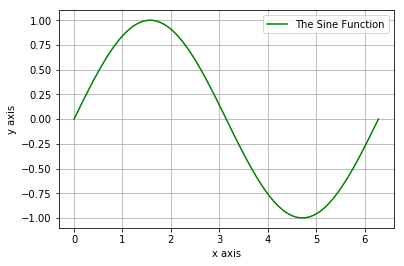
\includegraphics[width=0.7\columnwidth]{Images/matplotlib_1.png}
    \caption{The sine function on $x\in [0,2\pi]$, colored greed, with a grid, and with a
    legend.}
    \label{fig:matplotlib_1}
\end{figure}

\begin{example}[Overlayed Plots with MatPlotLib]
    Now let's do a second example, but this time we want to show four different plots on
    top of each other.  When you start a figure, \texttt{matplotlib} is expecting all of
    those plots to be layered on top of each other.  For MATLAB users, this means that you
    do not need the \texttt{hold on} command since it is automatically ``on''.  

In this example we will plot
$$y_0 = \sin(2\pi x) \quad y_1 = \cos(2 \pi x) \quad y_2 = y_0 + y_1 \quad \text{and} \quad y_3 = y_0 - y_1$$
on the domain $x \in [0,1]$ with 100 equally spaced points.  We'll give each of the plots a different line style, built a legend, put a grid on the plot, and give axis labels.

\bcode
\begin{lstlisting}
# We really don't need to import the packages again, 
# but for completeness of the example let's do it anyway.
import numpy as np
import matplotlib.pyplot as plt
%matplotlib inline

# build the x and y values
x = np.linspace(0,1,100)
y0 = np.sin(2*np.pi*x)
y1 = np.cos(2*np.pi*x)
y2 = y0 + y1
y3 = y0 - y1

# plot each of the functions (notice that they will be on the same axes)
plt.plot(x, y0, 'b-.', label=r"$y_0 = \sin(2\pi x)$")
plt.plot(x, y1, 'r--', label=r"$y_1 = \cos(2\pi x)$")
plt.plot(x, y2, 'g:', label=r"$y_2 = y_0 + y_1$")
plt.plot(x, y3, 'k-', label=r"$y_3 = y_0 - y_1$")

# put in a grid, legend, title, and axis labels
plt.grid()
plt.legend()
plt.title("Awesome Title")
plt.xlabel('x axis label')
plt.ylabel('y axis label')
plt.show()
\end{lstlisting}
The resulting plot can be seen in Figure \ref{fig:matplotlib_2}
\end{example}


\begin{figure}[ht!]
    \centering
    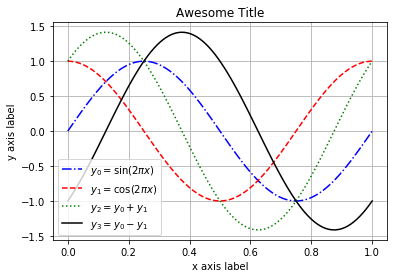
\includegraphics[width=0.7\columnwidth]{Images/matplotlib_2.png}
    \caption{Several trigonometric functions on the same axes.}
    \label{fig:matplotlib_2}
\end{figure}

Notice in Figure \ref{fig:matplotlib_2} that the legend was placed automatically.  There
are ways to control the placement of the legend if you wish, but for now just let Python
and \texttt{matplotlib} have control over the placement.

\begin{example}[Same Plot, Different Code]
    Now let's create the same plot as in Figure \ref{fig:matplotlib_2} with slightly different code.  The \texttt{plot}
    command can take several $(x, y)$ pairs in the same line of code.  This can really
    shrink the amount of coding that you have to do when plotting several functions on top
    of each other.

\bcode
\begin{lstlisting}
# The next line of code does all of the plotting of all of the functions.
# Notice the order: x, y, color and line style, repeat
plt.plot(x, y0, 'b-.', x, y1, 'r--', x, y2, 'g:', x, y3, 'k-')

plt.grid()
plt.legend([r"$y_0 = \sin(2\pi x)$",r"$y_1 = \cos(2\pi x)$",\
            r"$y_2 = y_0 + y_1$",r"$y_3 = y_0 - y_1$"])
plt.title("Awesome Title")
plt.xlabel('x axis label')
plt.ylabel('y axis label')
plt.show()
\end{lstlisting}
    
\end{example}


\begin{problem}
    Plot the functions $f(x) = x^2$, $g(x) = x^3$, and $h(x) = x^4$ on the same axes.  Use the domain $x \in [0,1]$ and the range $y \in [0,1]$.  Put a grid, a legend, a title, and appropriate labels on the axes.
\end{problem}


\subsection{Subplots}
It is often very handy to place plots side-by-side or as some array of plots.  The
\texttt{subplots} command allows us that control.  The main idea is that we are setting up
a matrix of blank plot and then populating the axes with the plots that we want.

\begin{example}[First Subplot Example]
    Let's repeat the previous exercise (which produced Figure \ref{fig:matplotlib_2}), but
    this time we will put each of the plots in its own subplot.  There are a few extra
    coding quirks that come along with building subplots so we'll highlight each block of
    code separately.

    \begin{itemize}
        \item First we set up the plot area with \texttt{plt.subplots()}.  The first two inputs
            to the \texttt{subplots} command are the number of rows and the number of
            columns in your plot array.  For the first example we will do 2 rows of plots
            with 2 columns -- so there are four plots total. The last input for the
            \texttt{subplots} command is the size of the figure (this is really just so
            that it shows up well in Jupyter Notebooks -- spend some time playing with the
            figure size to get it to look right).
        \item Then we build each plot individually telling \texttt{matplotlib} which axes
            to use for each of the things in the plots.
        \item Notice the small differences in how we set the titles and labels
        \item In this example we are setting the $y$-axis to the interval $[-2,2]$ for
            consistency across all of the plots.
    \end{itemize}

\bcode
\begin{lstlisting}
# set up the blank matrix of plots
fig, axes = plt.subplots(nrows = 2, ncols = 2, figsize = (10,5))

# Build the first plot
axes[0,0].plot(x, y0, 'b-.')
axes[0,0].grid()
axes[0,0].set_title(r"$y_0 = \sin(2\pi x)$")
axes[0,0].set_ylim(-2,2)
axes[0,0].set_xlabel("x")
axes[0,0].set_ylabel("y")

# Build the second plot
axes[0,1].plot(x, y1, 'r--')
axes[0,1].grid()
axes[0,1].set_title(r"$y_1 = \cos(2\pi x)$")
axes[0,1].set_ylim(-2,2)
axes[0,1].set_xlabel("x")
axes[0,1].set_ylabel("y")

# Build the first plot
axes[1,0].plot(x, y2, 'g:')
axes[1,0].grid()
axes[1,0].set_title(r"$y_2 = y_0 + y_1$")
axes[1,0].set_ylim(-2,2)
axes[1,0].set_xlabel("x")
axes[1,0].set_ylabel("y")

# Build the first plot
axes[1,1].plot(x, y3, 'k-')
axes[1,1].grid()
axes[1,1].set_title(r"$y_3 = y_0 - y_1$")
axes[1,1].set_ylim(-2,2)
axes[1,1].set_xlabel("x")
axes[1,1].set_ylabel("y")

fig.tight_layout()
\end{lstlisting}
The resulting plot can be seen in Figure \ref{fig:matplotlib_3}. The
\texttt{fig.tight\_layout()} command makes the plot labels a bit more readable in this
instance (again, something you can play with).
\end{example}


\begin{figure}[ht!]
    \centering
    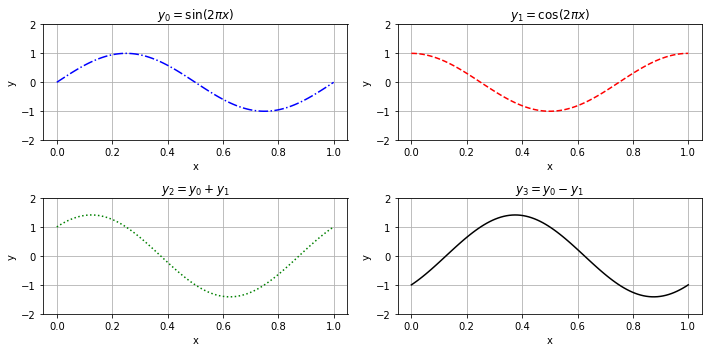
\includegraphics[width=0.95\columnwidth]{Images/matplotlib_3.png}
    \caption{The trigonometric functions with a $2\times 2$ matrix of subplots.}
    \label{fig:matplotlib_3}
\end{figure}

\begin{problem}
    Put the functions $f(x) = x^2$, $g(x) = x^3$ and $h(x) = x^4$ in a subplot environment with 1 row and 3 columns of plots.  Use the unit interval as the domain and range for all three plot, but sure that each plot has a grid, appropriate labels, an appropriate title, and the overall figure has a title.
\end{problem}


\subsection{Logarithmic Scaling with \texttt{semilogy}, \texttt{semilogx}, and
\texttt{loglog}}
It is occasionally useful to scale an axis logarithmically.  This arises most often when
we're examining an exponential function, or some other function, that is close to zero for
much of the domain.  Scaling logarithmically allows us to see how small the function is
getting in orders of magnitude instead of as a raw real number.

\begin{example}
    In this example we'll plot the function $y = 10^{-0.01x}$ on a regular (linear) scale
    and on a logarithmic scale on the $y$ axis.  Use the interval $[0,500]$ as a domain.

\bcode
\begin{lstlisting}
x = np.linspace(0,500,1000)
y = 10**(-0.01*x)
fig, axis = plt.subplots(1,2, figsize = (10,5))

axis[0].plot(x,y, 'r')
axis[0].grid()
axis[0].set_title("Linearly scaled y axis")
axis[0].set_xlabel("x")
axis[0].set_ylabel("y")

axis[1].semilogy(x,y, 'k--')
axis[1].grid()
axis[1].set_title("Logarithmically scaled y axis")
axis[1].set_xlabel("x")
axis[1].set_ylabel("Log(y)")
\end{lstlisting}
The output for this code can be seen in Figure \ref{fig:matplotlib_4}.

It should be noted that the same result can be achieved using the \texttt{yscale} command
along with the \texttt{plot} command instead of using the \texttt{semilogy} command.  Pay
careful attention to the subtle changes in the following code.

\bcode
\begin{lstlisting}
x = np.linspace(0,500,1000)
y = 10**(-0.01*x)
fig, axis = plt.subplots(1,2, figsize = (10,5))

axis[0].plot(x,y, 'r')
axis[0].grid()
axis[0].set_title("Linearly scaled y axis")
axis[0].set_xlabel("x")
axis[0].set_ylabel("y")

axis[1].plot(x,y, 'k--') # <----- Notice the change here
axis[1].set_yscale("log") # <----- And we added this line
axis[1].grid()
axis[1].set_title("Logarithmically scaled y axis")
axis[1].set_xlabel("x")
axis[1].set_ylabel("Log(y)")
\end{lstlisting}
\end{example}

\begin{figure}[ht!]
    \centering
    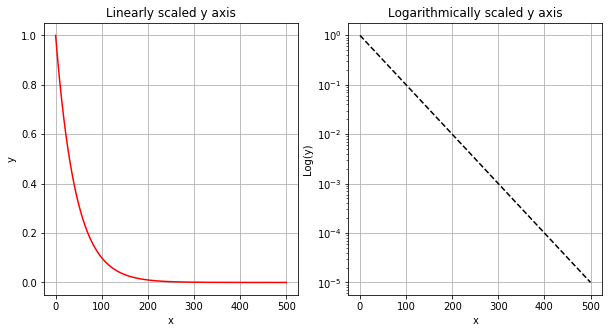
\includegraphics[width=0.9\columnwidth]{Images/matplotlib_4.png}
    \caption{The left-hand plot shows the exponential function $y = 10^{-0.01x}$ and the
right-hand side shows the same plot with the $y$ axis scaled logarithmically.}
    \label{fig:matplotlib_4}
\end{figure}


\begin{problem}
    Plot the function $f(x) = x^3$ for $x \in [0,1]$ on linearly scaled axes, logarithmic
    axis in the $y$ direction, logarithmically scaled axes in the $x$ direction, and a
    log-log plot with logarithmic scaling on both axes.  Use \texttt{subplots} to put your plots side-by-side.  Give appropriate labels, titles, etc.  
\end{problem}

\section{Symbolic Algebra and Calculus with \texttt{sympy}}
In this section we will learn the tools necessary to do symbolic mathematics in Python.
The relevant package is \texttt{sympy} (symbolic python) and it works much like
Mathematica, Maple, or MATLAB's symbolic toolbox.  That being said, Mathematica and Maple
are designed to do symbolic computation in the fastest and best possible ways, so in some
sense, \texttt{sympy} is a little step-sibling to these much bigger pieces of software.
Remember: Python is free, and this is a book on numerical analysis \ldots

For the sake of convenience we will load \texttt{matplotlib} so we can plot a few things
along the way.  

\bcode
\begin{lstlisting}
import matplotlib.pyplot as plt
%matplotlib inline
\end{lstlisting}

Let's import \texttt{sympy} in the usual way.  We will use the nickname \texttt{sp} (just
like we used \texttt{np} for \texttt{numpy}).  This is not a standard nickname in the
Python literature, but it will suffice for our purposes.

\bcode
\begin{lstlisting}
import sympy as sp
# The directory of sympy is full of stuff.  
# Uncomment the next line and run the code to see what you're getting.
# print(dir(sp))

sp.init_printing() # This allows for a more LaTeX style output
\end{lstlisting}
The last line of the previous block of code is again just for Jupyter Notebooks.  We want
to allow for some beautiful styling of the output of these symbolic calculations and this
is the line that allows Jupyter to do it.



\subsection{Symbolic Variables with \texttt{symbols}}
When you are working with symbolic variables you have to tell Python that that's what
you're doing.  In other words, we actually have to type-cast the variables when we name
them.  Otherwise Python won't know what to do with them.

Let's define the variable $x$ as a symbolic variable.  Then we'll define a few symbolic
expressions that use $x$ as a variable.

\bcode
\begin{lstlisting}
x = sp.Symbol('x') # note the capitalization
\end{lstlisting}

Now we'll define the function $f(x) = (x+2)^3$ and spend the next few examples playing
with it.

\bcode
\begin{lstlisting}
f = (x+2)**3 # A symbolic function
f
\end{lstlisting}
The output of these lines of code is the nicely formatted symbolic expression $\displaystyle
(x+2)^3$.

Be careful that you are using symbolically defined function along with your symbols.  For example, see the code below:

\bcode
\begin{lstlisting}
# g = sin(x) # this line gives an error since it doesn't know which "sine" function to use.
g = sp.sin(x) # this one works
g
\end{lstlisting}
The output of these lines of code is the symbolic expression $\sin(x)$.

\subsection{Symbolic Algebra}
One of the primary purposes of doing symbolic programming is to do symbolic algebra (the
other is typically symbolic calculus).  In this section we'll look at a few of the common
algebraic exercises that can be handled with \texttt{sympy}.

\begin{example}[Expand a Polynomial]
    Expand the function $f(x) = (x+2)^3$.  In other words, multiply this out fully so that
    it is a sum or difference of monomials instead of the cube of a binomial.

\bcode
\begin{lstlisting}
f = (x+2)**3
sp.expand(f) # do the multiplication to expand the polynomial
\end{lstlisting}
The output of these lines of code is the expression $x^{3} + 6 x^{2} + 12 x + 8$.
\end{example}

\begin{example}[Factor a Polynomial]
    We will factor the polynomial $h(x) = x^2 + 4x + 3$.

\bcode
\begin{lstlisting}
h = x**2 + 4*x + 3
sp.factor(h) # factor this polynomial
\end{lstlisting}
The output of this function is the expression $\left(x + 1\right) \left(x + 3\right)$.
\end{example}

\begin{example}[Trig Expansion]
    The \texttt{sympy} package knows how to work with trigonometric identities.  In this
    example we show how \texttt{sympy} expands $\sin(a+b)$.

\bcode
\begin{lstlisting}
a, b = sp.symbols('a b')
j = sp.sin(a+b)
sp.expand(j, trig=True) # Trig identities are built in!
\end{lstlisting}
The output of these linse of code is the expression $\displaystyle \sin{\left(a
\right)} \cos{\left(b \right)} + \sin{\left(b \right)} \cos{\left(a \right)}$
\end{example}

\begin{example}[Simplifying Algebraic Expressions]
    In this example we will simplify the function $g(x) = x^3 + 5x^3 + 12x^2 +1$.

\bcode
\begin{lstlisting}
g = x**3 + 5*x**3 + 12*x**2 + 1
sp.simplify(g) # Simplify some algebraic expression
\end{lstlisting}
The output of these lines of code is the expression $6 x^{3} + 12 x^{2} + 1$.
\end{example}

\begin{example}[Simplifying Trig Expressions]
    In this example we'll simplify an expression that involves trigonometry.

\bcode
\begin{lstlisting}
sp.simplify( sp.sin(x) / sp.cos(x)) # simplify a trig expression.
\end{lstlisting}
The output of this line of code is the expression $\tan(x)$ as expected.
\end{example}

The primary goal of many algebra problems is to solve an equation.  We will dedicate more
time to algebraic equation solving later in this section, but the following example gives
a simple example of how it works in \texttt{sympy}.

\begin{example}[Simple Equation Solving]
    We want to solve the equation $x^2 + 4x + 3 = 0$ for $x$.

\bcode
\begin{lstlisting}
h = x**2 + 4*x + 3
sp.solve(h,x)
\end{lstlisting}
\boutput
\begin{lstlisting}
[-3, -1]
\end{lstlisting}
As expected, the roots of the function $h(x)$ are $x=-3$ and $x=1$ since $h(x)$ factors
into $h(x) = (x+3)(x-1)$.
    
\end{example}

\subsection{Symbolic Function Evaluation}
In \texttt{sympy} we cannot simply just evaluate functions as we would on paper.  Let's
say we have the function $f(x)= (x+2)^3$ and we want to find $f(5)$.  We would say that we
``substitute 5 into f for x'', and that is exactly what we have to tell Python.
Unfortunately we cannot just write ``f(5)'' since that would mean that ``f'' is a Python
function and we are sending the number 5 into that function.  This is an unfortunate
double-use of the word ``function'', but stop and think about it for a second: When we
write \texttt{f = (x+2)**3} we are just telling Python that \texttt{f} is a symolic
expression in terms of the symbol \texttt{x}, but we did not use \texttt{def} to define it
as a function as we did for all other function.

The following code is what the mathematicians in us would like to do:
\bcode
\begin{lstlisting}
f = (x+2)**3
f(5) # This gives an error!
\end{lstlisting}

\ldots but this is how it should be done:
\bcode
\begin{lstlisting}
f.subs(x,5) # This actually substitutes 5 for x in f
\end{lstlisting}
\boutput
\begin{lstlisting}
343
\end{lstlisting}


\subsection{Symbolic Calculus}
The \texttt{sympy} package has routines to take symbolic derivatives, antiderivatives,
limits, and Taylor series just like other computer algebra systems.  

\subsubsection{Derivatives}
The \texttt{diff} command in \texttt{sympy} does differentiation.
\begin{lstlisting}
sp.diff(function, variable, [order])
\end{lstlisting}
Take careful note that \texttt{diff} is defined both in \texttt{sympy} and in
\texttt{numpy}.  That means that there are symbolic and numerical routines for taking
derivatives in Python \ldots and we need to tell our instance of Python which one we're working with every time we use it.  

\begin{example}[Symbolic Differentiation]
    In this example we'll differentiate the function $f(x) = (x+2)^3$.

\bcode
\begin{lstlisting}
import sympy as sp # we already did this above, but let's do it again for clarity
x = sp.Symbol('x') # Define the symbol x
f = (x+2)**3 # Define a symbolic function f(x) = (x+2)^3
df = sp.diff(f,x) # Take the derivative of f and call it "df"
print("f(x) = ", f)
print("f'(x) = ",df)
print("f'(x) = ", sp.expand(df))
\end{lstlisting}
\boutput
\begin{lstlisting}
f(x) =  (x + 2)**3
f'(x) =  3*(x + 2)**2
f'(x) =  3*x**2 + 12*x + 12
\end{lstlisting}

Now let's get the first, second, third, and fourth derivatives of the function \texttt{f}.

\bcode
\begin{lstlisting}
df = sp.diff(f,x,1) # first derivative
ddf = sp.diff(f,x,2) # second deriative
dddf = sp.diff(f,x,3) # third deriative
ddddf = sp.diff(f,x,4) # fourth deriative
print("f'(x) = ",df)
print("f''(x) = ",sp.simplify(ddf))
print("f'''(x) = ",sp.simplify(dddf))
print("f''''(x) = ",sp.simplify(ddddf))
\end{lstlisting}
\boutput
\begin{lstlisting}
f'(x) =  3*(x + 2)**2
f''(x) =  6*x + 12
f'''(x) =  6
f''''(x) =  0
\end{lstlisting}
\end{example}

\begin{example}[Partial Derivatives]
    Now let's do some partial derivatives.  The \texttt{diff} command is still the right
    tool.  You just have to tell it which variable you're working with.

\bcode
\begin{lstlisting}
x, y = sp.symbols('x y') # Define the symbols
f = sp.sin(x*y) + sp.cos(x**2) # Define the function
fx = sp.diff(f,x)
fy = sp.diff(f,y)
print("f(x,y) = ", f)
print("f_x(x,y) = ", fx)
print("f_y(x,y) = ", fy)
\end{lstlisting}
\boutput
\begin{lstlisting}
f(x,y) =  sin(x*y) + cos(x**2)
f_x(x,y) =  -2*x*sin(x**2) + y*cos(x*y)
f_y(x,y) =  x*cos(x*y)
\end{lstlisting}
\end{example}

\begin{example}[\LaTeX\ from Symbolic Expressions]
    It is worth noting that when you have a symbolically defined function you can ask
    sympy to give you the \LaTeX\ code for the symbolic function so you can use it when you write about it.

\bcode
\begin{lstlisting}
sp.latex(f)
\end{lstlisting}
\boutput
\begin{lstlisting}
'\\sin{\\left(x y \\right)} + \\cos{\\left(x^{2} \\right)}'
\end{lstlisting}
\end{example}

\subsubsection{Integrals}
For integration, the \texttt{integrate} tool is the command for the job
\begin{lstlisting}
sp.integrate(function, variable) # antiderivative
sp.integrate(function, (variable, lower, upper)) # definite integral
\end{lstlisting}
The
\texttt{integrate} command in \texttt{sympy} accepts a symbolically defined function along
with the variable of integration and optional bounds.  If the bounds aren't given then the
command finds the antiderivative.  Otherwise it finds the definite integral.

\begin{example}[An Antiderivative]
    Find the antiderivative of the function $f(x) = (x+2)^3$.

\bcode
\begin{lstlisting}
import sympy as sp 
x = sp.Symbol('x')
f = (x+2)**3
F = sp.integrate(f,x)
F
\end{lstlisting}
The output of these lines of code is the expression $\frac{x^{4}}{4} + 2 x^{3} + 6 x^{2}
+ 8 x$ which is indeed the antiderivative.  We can ask \texttt{sympy} to factor the result
with 

\bcode
\begin{lstlisting}
sp.factor(F)
\end{lstlisting}
which results in the expression $\displaystyle \frac{x \left(x + 4\right) \left(x^{2}
+ 4 x + 8\right)}{4}$
\end{example}

\begin{example}[Another Antiderivative]
    Consider the multivariable antiderivative
    \[ \int \sin(xy) + \cos(x) dx.\]
    The \texttt{sympy} package deals with the second variable just as it should.  

\bcode
\begin{lstlisting}
g = sp.sin(x*y) + sp.cos(x)
G = sp.integrate(g,x) 
G 
\end{lstlisting}
These lines of code result in the output 
\[ \begin{cases} - \frac{\cos{\left(x y \right)}}{y} & \text{for}\: y \neq 0 \\0 & \text{otherwise} \end{cases} + \sin{\left(x \right)}  \]
so it is apparent that \texttt{sympy} was sensitive to the fact that there was trouble at
$y=0$ and took care of it with a piecewise function.

\end{example}

\begin{example}[A Definite Integral]
    Consider the integral $$\int_0^\pi \sin(x) dx.$$
    Notice that the variable and the bounds are sent to the \texttt{integrate} command as
    a tuple.  Furthermore, notice that we had to send the symbolic version of $\pi$
    instead of any other version (e.g. \texttt{numpy}).

\bcode
\begin{lstlisting}
sp.integrate( sp.sin(x), (x,0,sp.pi))
\end{lstlisting}
This line of code results in $2$; the correct definite integral.
\end{example}

\begin{example}[A Tougher Definite Integral]
    This is a fun one.  Let's do the definite integral
$$ \int_{-\infty}^\infty e^{-x^2} dx.$$
We have to use the ``infinity'' symbol from \texttt{sympy}.  It is two lower-case O's next
to each other: \texttt{oo}.  It kind of looks like and infinity I suppose.  

\bcode
\begin{lstlisting}
sp.integrate( sp.exp(-x**2) , (x, -sp.oo, sp.oo))
\end{lstlisting}
which results in the value $\sqrt{\pi}$ \ldots which is simply a fun integral.

\end{example}

\subsubsection{Limits}
The \texttt{limit} command in \texttt{sympy} takes symbolic limits
\begin{lstlisting}
sp.limit(function, variable, value, [direction])
\end{lstlisting}
The direction (left or right) is optional and if you leave it off then the limit is
considered from both directions.

\begin{example}[Symbolic Limit]
    Let's take the limit
$$\lim_{x \to 0} \frac{\sin(x)}{x}.$$

\bcode
\begin{lstlisting}
sp.limit( sp.sin(x)/x, x, 0)
\end{lstlisting}
which gives us the value 1.
\end{example}

\begin{example}[Difference Quotient]
    Let's do the difference quotient
$$\lim_{h \to 0} \frac{ f(x+h) - f(x)}{h}$$
for the function $f(x) = (x+2)^3$.  Taking the limit should give the derivative so we'll
check that the \texttt{diff} command gives us the same thing using \texttt{==} \ldots warning!

\bcode
\begin{lstlisting}
f = (x+2)**3
print(sp.diff(f,x))
h = sp.Symbol('h')
df = sp.limit( (f.subs(x,x+h) - f) / h , h , 0 )
print(df)
print(df == sp.diff(f,x)) # notice that these are not "symbolically" equatl
print(df == sp.expand(sp.diff(f,x))) # but these are
\end{lstlisting}
\boutput
\begin{lstlisting}
3*(x + 2)**2
3*x**2 + 12*x + 12
False
True
\end{lstlisting}
Notice that when we check to see if two symbolic functions are equal they must be in the
same exact symbolic form.  Otherwise \texttt{sympy} won't recognize them as actually being
equal even though they are mathematically equivalent.
\end{example}

\begin{problem}
    Define the function $f(x) = 3x^2 + x\sin(x^2)$ symbolically and then do the following:

    \begin{enumerate}
        \item Evaluate the function at $x=2$ and get symbolic and numerical answers.
        \item Take the first and second derivative
        \item Take the antiderivative
        \item Find the definite integral from 0 to 1
        \item Find the limit as $x$ goes to 3
    \end{enumerate}
\end{problem}

\subsubsection{Taylor Series}
The \texttt{sympy} package has a tool for expanding Taylor Series of symbolic functions.  
\begin{lstlisting}
sp.series( function, variable, [center], [num terms])
\end{lstlisting}
The center defaults to $0$ and the number of terms defaults to $5$.  

\begin{example}[A Taylor Series Expansion]
    Find the Taylor series for $f(x) = e^x$ centered at $x=0$ and centered at $x=1$.  

\bcode
\begin{lstlisting}
sp.series( sp.exp(x),x)
\end{lstlisting}
gives the output $\displaystyle 1 + x + \frac{x^{2}}{2} + \frac{x^{3}}{6} +
\frac{x^{4}}{24} + \frac{x^{5}}{120} + \mathcal{O}\left(x^{6}\right).$

\bcode
\begin{lstlisting}
sp.series( sp.exp(x), x, 1) # expand at x=1
\end{lstlisting}
gives the output 
\[ e + e \left(x - 1\right) + \frac{e \left(x -
    1\right)^{2}}{2} + \frac{e \left(x - 1\right)^{3}}{6} + \frac{e \left(x -
        1\right)^{4}}{24} + \frac{e \left(x - 1\right)^{5}}{120} + \mathcal{O}\left(\left(x -
    1\right)^{6}; x\rightarrow 1\right) \]

Finally, if we want more terms then we can send the number of desired terms to the
\texttt{series} command.

\bcode
\begin{lstlisting}
sp.series( sp.exp(x), x, 0, 10) # expand at x=0 and give 10 terms
\end{lstlisting}
gives the output
\[ 1 + x + \frac{x^{2}}{2} + \frac{x^{3}}{6} + \frac{x^{4}}{24} + \frac{x^{5}}{120} +
    \frac{x^{6}}{720} + \frac{x^{7}}{5040} + \frac{x^{8}}{40320} +
\frac{x^{9}}{362880} + \mathcal{O}\left(x^{10}\right). \]
\end{example}

\subsection{Solving Equations Symbolically}
One of the big reasons to use a symbolic toolboxes such as \texttt{sympy} is to solve
algebraic equations exactly.  This isn't always going to be possible, but when it is we
get some nice results.  The \texttt{solve} command in \texttt{sympy} is the tool for the job.
\begin{lstlisting}
sp.solve( equation, variable )
\end{lstlisting}
The equation doesn't actually need to be the whole equation.  For any equation-solving
problem we can always reframe it so that we are solving $f(x) = 0$ by subtracting the
right-hand side of the equation to the left-hand side.  Hence we can leave the equal sign
and the zero off and \texttt{sympy} understands what we're doing.

\begin{example}[Solve Equation Symbolically]
    Let's solve the equation $x^2 - 2 = 0$ for $x$.  We know that the roots are $\pm \sqrt{2}$ so this should be pretty trivial for a symbolic solver.

\bcode
\begin{lstlisting}
sp.solve( x**2 - 2, x)
\end{lstlisting}
gives the output
$\displaystyle \left[ -\sqrt{2}, \sqrt{2} \right]$.
\end{example}

\begin{example}[A Slightly More Challenging Equation Solving Problem]
    Now let's solve the equation $x^4 - x^2 - 1= 0$ for $x$.  You might recognize this as
    a quadratic equation in disguise so you can definitely do it by hand ... if you want
    to.  (You could also recognize that this equation is related to the golden ratio!)

\bcode
\begin{lstlisting}
sp.solve( x**4 - x**2 - 1, x)
\end{lstlisting}
which gives the output
\[ \left[ - i \sqrt{- \frac{1}{2} + \frac{\sqrt{5}}{2}}, \  i \sqrt{- \frac{1}{2} + \frac{\sqrt{5}}{2}}, \  - \sqrt{\frac{1}{2} + \frac{\sqrt{5}}{2}}, \  \sqrt{\frac{1}{2} + \frac{\sqrt{5}}{2}}\right] \]
Notice that \texttt{sympy} has no problem dealing with the complex roots. 
\end{example}

In the previous example the answers may be a bit hard to read due to their symbolic form.
This is particularly true for far more complicated equation solving problems.  The next
example shows how you can loop through the solutions and then print them in decimal form
so they are a bit more readable.

\begin{example}[Converting Symbolic Answers to Floating Point]
   We will again solve the equation   $x^4 - x^2 - 1= 0$ for $x$, but this time we will
   output the answers as floating point decimals.  We are using the \texttt{N} command to
   convert from symbolic to numerical.

\bcode
\begin{lstlisting}
soln = sp.solve( x**4 - x**2 - 1, x)
for j in range(0, len(soln)):
    print(sp.N(soln[j]))
\end{lstlisting}
\boutput
\begin{lstlisting}
-0.786151377757423*I
0.786151377757423*I
-1.27201964951407
1.27201964951407
\end{lstlisting}
\end{example}

The \texttt{N} command gives a numerical approximation for a symbolic expression (this is
taken straight from Mathematica!).

\begin{problem}
    Give the exact and floating point solutions to the equation $x^4 - x^2 - x + 5 = 0$.
\end{problem}


When you want to solve a symbolic equation numerically you can use the \texttt{nsolve}
command.  This will do something like Newton's method in the background.  You need to give
it a starting point where it can look for you the solution to your equation.  
\begin{lstlisting}
sp.nsolve( equation, variable, intial guess )
\end{lstlisting}

\begin{example}[Numerical Solve on a Symbolically Defined Equation]
    Let's solve the equation $x^3 - x^2 - 2$ for $x$ both symbolically and numerically.
    The numerical solution with \texttt{nsolve} will search for the solution near $x=1$.

\bcode
\begin{lstlisting}
sp.solve(x**3 - x**2 - 2, x, 1) # symbolic solution
\end{lstlisting}
gives the exact solution
\begin{flalign*}
\left[ \frac{1}{3} + \left(- \frac{1}{2} - \frac{\sqrt{3} i}{2}\right)
    \sqrt[3]{\frac{\sqrt{87}}{9} + \frac{28}{27}} + \frac{1}{9 \left(- \frac{1}{2} -
    \frac{\sqrt{3} i}{2}\right) \sqrt[3]{\frac{\sqrt{87}}{9} + \frac{28}{27}}}, \right. \\
    \frac{1}{3} + \frac{1}{9 \left(- \frac{1}{2} + \frac{\sqrt{3} i}{2}\right)
    \sqrt[3]{\frac{\sqrt{87}}{9} + \frac{28}{27}}} + \left(- \frac{1}{2} + \frac{\sqrt{3}
i}{2}\right) \sqrt[3]{\frac{\sqrt{87}}{9} + \frac{28}{27}}, \\
\left. \frac{1}{9 \sqrt[3]{\frac{\sqrt{87}}{9} + \frac{28}{27}}} + \frac{1}{3} + \sqrt[3]{\frac{\sqrt{87}}{9} + \frac{28}{27}}\right]
\end{flalign*}
which is rather challenging to read.  We can give all of the floating point approximations
with the following code.

\bcode
\begin{lstlisting}
print("First Solution: ",sp.N(ExactSoln[0]))
print("Second Solution: ",sp.N(ExactSoln[1]))
print("Third Solution: ",sp.N(ExactSoln[2]))
\end{lstlisting}
\boutput
\begin{lstlisting}
First Solution:  -0.347810384779931 - 1.02885225413669*I
Second Solution:  -0.347810384779931 + 1.02885225413669*I
Third Solution:  1.69562076955986
\end{lstlisting}

If we were only looking for the floating point real solution near $x=1$ then we could just
use \texttt{nsolve}.

\bcode
\begin{lstlisting}
sp.nsolve(x**3 - x**2 - 2, x, 1)
\end{lstlisting}
\boutput
\begin{lstlisting}
1.69562076955986
\end{lstlisting}
\end{example}


\begin{problem}
    Solve the equation 
$$x^3 \ln(x) = 7$$
and give your answer both symbolically and numerically.
\end{problem}

\subsection{Symbolic Plotting}
In this final section we will show how to make plots of symbolically defined functions.
Be careful here.  There are times when you want to plot a symbolically defined function
and there are times when you want to plot data.  
\begin{lstlisting}
sp.plot( function, (variable, left, right) )
\end{lstlisting}
It is easy to get confused since they
both use the \texttt{plot} function in their own packages (\texttt{sympy} and
\texttt{matplotlib} respectively).

Note: For MATLAB users, the \texttt{sympy.plot} command is similar to MATLAB's
\texttt{ezplot} command.

In numerical analysis we don't often need to make plots of symbolically defined functions.
There is more that could be said about \texttt{sympy}'s plotting routine, but since it
won't be used often in this text it doesn't seem necessary to give those details here.
When you need to make a plot just make a careful consideration as to whether you need a
symbolic plot (with \texttt{sympy}) or a plot of data points (with \texttt{matplotlib}).

\begin{example}[A Symbolic Plot]
    Let's get a quick plot of the function $f(x) = (x+2)^3$ on the domain $x \in [-5,2]$.

\bcode
\begin{lstlisting}
import sympy as sp
x = sp.Symbol('x')
f = (x+2)**3
sp.plot(f,(x,-5,2))
\end{lstlisting}
The output for which can be seen in Figure \ref{fig:sympy_plot_1}.
\end{example}

\begin{figure}[ht!]
    \centering
    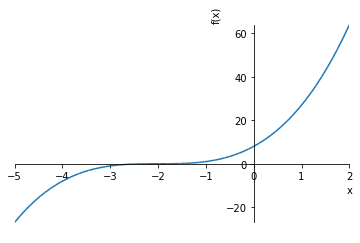
\includegraphics[width=0.6\columnwidth]{Images/sympy_plot_1.png}
    \caption{A plot of $f(x) = (x+2)^3$ on the domain $x \in [-5,2]$ created with
        \texttt{sympy.plot}.}
    \label{fig:sympy_plot_1}
\end{figure}

Multiple plots can be done at the same time with the \texttt{sympy.plot} command.

\begin{example}
    Plot $f(x) = (x+2)^3$ and $g(x) = 20\cos(x)$ on the same axes on the domain $x \in
    [-5,2]$.

\bcode
\begin{lstlisting}
import sympy as sp
x = sp.Symbol('x')
f = (x+2)**3
g = 20*sp.cos(x)
sp.plot(f, g, (x,-5,2))
\end{lstlisting}
The output for which can be seen in Figure \ref{fig:sympy_plot_2}
\end{example}

\begin{figure}[ht!]
    \centering
    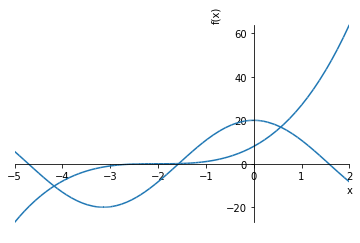
\includegraphics[width=0.6\columnwidth]{Images/sympy_plot_2.png}
    \caption{Two plots on top of eachother created with \texttt{sympy.plot}.}
    \label{fig:sympy_plot_2}
\end{figure}


\begin{problem}
    Make a symbolic plot of the function $f(x) = x^3 \ln(x) - 7$ on the domain $[0,3]$.
\end{problem}



